%%*************************************************************************
%% Legal Notice:
%% This code is offered as-is without any warranty either expressed or
%% implied; without even the implied warranty of MERCHANTABILITY or
%% FITNESS FOR A PARTICULAR PURPOSE! 
%% User assumes all risk.
%% In no event shall IEEE or any contributor to this code be liable for
%% any damages or losses, including, but not limited to, incidental,
%% consequential, or any other damages, resulting from the use or misuse
%% of any information contained here.
%%
%% All comments are the opinions of their respective authors and are not
%% necessarily endorsed by the IEEE.
%%
%% This work is distributed under the LaTeX Project Public License (LPPL)
%% ( http://www.latex-project.org/ ) version 1.3, and may be freely used,
%% distributed and modified. A copy of the LPPL, version 1.3, is included
%% in the base LaTeX documentation of all distributions of LaTeX released
%% 2003/12/01 or later.
%% Retain all contribution notices and credits.
%% ** Modified files should be clearly indicated as such, including  **
%% ** renaming them and changing author support contact information. **
%%
%% File list of work: IEEEtran.cls, IEEEtran_HOWTO.pdf, bare_adv.tex,
%%                    bare_conf.tex, bare_jrnl.tex, bare_jrnl_compsoc.tex
%%*************************************************************************
\documentclass[conference]{IEEEtran}

% *** GRAPHICS RELATED PACKAGES ***
\ifCLASSINFOpdf
   \usepackage[pdftex]{graphicx}
   \graphicspath{{img/}}
   \DeclareGraphicsExtensions{.pdf,.jpeg,.png}
\fi

% *** MATH PACKAGES ***
%
\usepackage[cmex10]{amsmath}
% A popular package from the American Mathematical Society that provides
% many useful and powerful commands for dealing with mathematics. If using
% it, be sure to load this package with the cmex10 option to ensure that
% only type 1 fonts will utilized at all point sizes. Without this option,
% it is possible that some math symbols, particularly those within
% footnotes, will be rendered in bitmap form which will result in a
% document that can not be IEEE Xplore compliant!
%
% Also, note that the amsmath package sets \interdisplaylinepenalty to 10000
% thus preventing page breaks from occurring within multiline equations. Use:
%\interdisplaylinepenalty=2500
% after loading amsmath to restore such page breaks as IEEEtran.cls normally
% does. amsmath.sty is already installed on most LaTeX systems. The latest
% version and documentation can be obtained at:
% http://www.ctan.org/tex-archive/macros/latex/required/amslatex/math/


% *** SPECIALIZED LIST PACKAGES ***
%
%\usepackage{algorithmic}
% algorithmic.sty was written by Peter Williams and Rogerio Brito.
% This package provides an algorithmic environment fo describing algorithms.
% You can use the algorithmic environment in-text or within a figure
% environment to provide for a floating algorithm. Do NOT use the algorithm
% floating environment provided by algorithm.sty (by the same authors) or
% algorithm2e.sty (by Christophe Fiorio) as IEEE does not use dedicated
% algorithm float types and packages that provide these will not provide
% correct IEEE style captions. The latest version and documentation of
% algorithmic.sty can be obtained at:
% http://www.ctan.org/tex-archive/macros/latex/contrib/algorithms/
% There is also a support site at:
% http://algorithms.berlios.de/index.html
% Also of interest may be the (relatively newer and more customizable)
% algorithmicx.sty package by Szasz Janos:
% http://www.ctan.org/tex-archive/macros/latex/contrib/algorithmicx/




% *** ALIGNMENT PACKAGES ***
%
%\usepackage{array}
% Frank Mittelbach's and David Carlisle's array.sty patches and improves
% the standard LaTeX2e array and tabular environments to provide better
% appearance and additional user controls. As the default LaTeX2e table
% generation code is lacking to the point of almost being broken with
% respect to the quality of the end results, all users are strongly
% advised to use an enhanced (at the very least that provided by array.sty)
% set of table tools. array.sty is already installed on most systems. The
% latest version and documentation can be obtained at:
% http://www.ctan.org/tex-archive/macros/latex/required/tools/


%\usepackage{mdwmath}
%\usepackage{mdwtab}
% Also highly recommended is Mark Wooding's extremely powerful MDW tools,
% especially mdwmath.sty and mdwtab.sty which are used to format equations
% and tables, respectively. The MDWtools set is already installed on most
% LaTeX systems. The lastest version and documentation is available at:
% http://www.ctan.org/tex-archive/macros/latex/contrib/mdwtools/



%\usepackage{eqparbox}
% Also of notable interest is Scott Pakin's eqparbox package for creating
% (automatically sized) equal width boxes - aka "natural width parboxes".
% Available at:
% http://www.ctan.org/tex-archive/macros/latex/contrib/eqparbox/


% *** FLOAT PACKAGES ***
%
%\usepackage{fixltx2e}
% fixltx2e, the successor to the earlier fix2col.sty, was written by
% Frank Mittelbach and David Carlisle. This package corrects a few problems
% in the LaTeX2e kernel, the most notable of which is that in current
% LaTeX2e releases, the ordering of single and double column floats is not
% guaranteed to be preserved. Thus, an unpatched LaTeX2e can allow a
% single column figure to be placed prior to an earlier double column
% figure. The latest version and documentation can be found at:
% http://www.ctan.org/tex-archive/macros/latex/base/



%\usepackage{stfloats}
% stfloats.sty was written by Sigitas Tolusis. This package gives LaTeX2e
% the ability to do double column floats at the bottom of the page as well
% as the top. (e.g., "\begin{figure*}[!b]" is not normally possible in
% LaTeX2e). It also provides a command:
%\fnbelowfloat
% to enable the placement of footnotes below bottom floats (the standard
% LaTeX2e kernel puts them above bottom floats). This is an invasive package
% which rewrites many portions of the LaTeX2e float routines. It may not work
% with other packages that modify the LaTeX2e float routines. The latest
% version and documentation can be obtained at:
% http://www.ctan.org/tex-archive/macros/latex/contrib/sttools/
% Documentation is contained in the stfloats.sty comments as well as in the
% presfull.pdf file. Do not use the stfloats baselinefloat ability as IEEE
% does not allow \baselineskip to stretch. Authors submitting work to the
% IEEE should note that IEEE rarely uses double column equations and
% that authors should try to avoid such use. Do not be tempted to use the
% cuted.sty or midfloat.sty packages (also by Sigitas Tolusis) as IEEE does
% not format its papers in such ways.





% *** PDF, URL AND HYPERLINK PACKAGES ***
\usepackage{url}
\usepackage[utf8]{inputenc}
%\usepackage[spanish]{babel}
\usepackage{booktabs}
\usepackage{listings}

\usepackage{tabularx}
% correct bad hyphenation here
\hyphenation{op-tical net-works semi-conduc-tor}


\begin{document}
%
% paper title
% can use linebreaks \\ within to get better formatting as desired
\title{Desambiguación semántica de autores sobre fuentes biblíograficas digitales}

% for over three affiliations, or if they all won't fit within the width
% of the page, use this alternative format:
% 
\author{\IEEEauthorblockN{Michael Shell\IEEEauthorrefmark{1},
Homer Simpson\IEEEauthorrefmark{2},	
James Kirk\IEEEauthorrefmark{3}, 
Montgomery Scott\IEEEauthorrefmark{4} and
Eldon Tyrell\IEEEauthorrefmark{5}}
\IEEEauthorblockA{Computer Science Department, Universidad de Cuenca,\\
Cuenca, Ecuador.}
\IEEEauthorblockA{\IEEEauthorrefmark{1}http://www.michaelshell.org/contact.html}
\IEEEauthorblockA{\IEEEauthorrefmark{2}homer@thesimpsons.com}
\IEEEauthorblockA{\IEEEauthorrefmark{3}james@thesimpsons.com}
\IEEEauthorblockA{\IEEEauthorrefmark{4}montgomery@thesimpsons.com}
\IEEEauthorblockA{\IEEEauthorrefmark{5}eldon@thesimpsons.com}}

% make the title area
\maketitle


\begin{abstract}
The abstract goes here.
\end{abstract}
% no keywords

\IEEEpeerreviewmaketitle

\section{Introducción}
\label{sec:introduccion}
%En las instituciones de educación superior (IES), así como en otras instituciones asociada como bibliotecas se almacenan una gran cantidad de producción científica y académica dentro de repositorios digitales. Esta producción está compuesta principalmente por los  recursos bibliográficos generados dentro de la institución tales como tesis, artículos, trabajos de pregrado o postgrado, entre otros, que reflejan el trabajo realizado tanto de profesores, investigadores como de alumnos dentro de estas instituciones. En la actualidad gracias a las tecnologías  semánticas y proyectos conjuntos de integración  dichos repositorios han dado un paso hacia el futuro, pasando de lo que comúnmente eran silos aislados de información, a formar parte de  una red de  repositorios accesibles para todo público a través de la web. Un ejemplo  de esto se puede apreciar en el trabajo realizado por el GTR\footnote{\url{http://gtrepositorios.cedia.org.ec/}} en Ecuador, que con el apoyo de la institución REDCEDIA\footnote{\url{https://www.cedia.edu.ec}} ha convertido y publicado los datos disponibles de un gran número de repositorios institucionales de universidades a un formato compatible con los  principios de Linked Data\footnote{cambiar: \url{Datahub.io}}. Este nuevo sistema de representación de  la información no solo  ha permitido que estos repositorios aislados  puedan ser accesibles de forma global e interoperable entre sí, sino que también  han dado un importante paso hacia la mejora en  la visibilidad  del trabajo institucional,  tanto a nivel interno  como interinstitucional. Mediante la aplicación de estas tecnologías ahora es más sencillo la detección trabajos conjuntos entre  universidades, verificar el aporte de investigadores en varias instituciones e incluso tener un rastreo de las actividades de un estudiante que puede seguir sus estudios posteriores (postgrado) en otras instituciones, entre otras.  Aunque, las ventajas de emplear estas tecnologías son evidentes, este incremento de información y su centralización ha traído consigo  nuevos retos a superar para sacar el máximo provecho de estas bases digitales. Uno de estos retos  consiste en  la dificultad para  la identificación plena de  los  autores,  provocado principalmente por la representación ambigua y variable de un autor al ser  representado únicamente por su nombre.   Esta práctica, común en el medio,  genera que las tareas de  reconocimiento o asignación  de autores con sus obras a través de varias fuentes o incluso sobre una misma fuente, sea una tarea compleja y laboriosa que en muchos casos es realizada de forma manual y en la mayoría de los casos  propensa a errores. Este es un problema común que se encuentra en bases digitales y es más laborioso conforme aumenta el número de autores y sus obras \cite{Lee:2007:YCC:1323688.1323690}. Este problema ha sido abordado  por múltiples trabajos  en la comunidad científica  bajo la denominación de desambiguación de nombres de autores (Author Name Disambiguation, AND).
Bibliotecas académicas almacenan en sus repositorios digitales una gran cantidad de recursos de producción científica y académica. Está información es ingresada manualmente o es extraída de bibliotecas digitales y desambiguar nombres de autores (Author Name Disambiguation, AND) es deseable porque ayuda, por ejemplo, a procesos de búsqueda cómo encontrar artículos publicados por una específica persona o en la integración de información; ésto es un desafío para bibliotecas digitales. Los usuarios normalmente tienen que tratar con resultados de una búsqueda para encontrar el autor correcto. Además, desambiguar nombres ayuda a realizar estudios bibliométricos debido a que existe una correcta atribución de trabajos científicos y también se puede descubrir nuevo conocimiento usando tecnicas de mineria de datos. 

%La ambigüedad de nombres puede ser a causa de varios factores como errores de ortografía, inconsistencias al ingresar datos, variaciones del nombre o uso de iniciales; estos factores pueden ser englobados en tres grupos. El primero es cuando varias personas comparten el mismo nombre (homónimos), en el segundo grupo están todas las representaciones del nombre de un autor (sinónimos) como por ejemplo ``Mauricio Espinoza'' y ``M. Espinoza'', y errores tipográficos o ortográficos se encuentran en el tercer grupo. Además del nombre, se puede extraer  otras características del autor que agreguen el conocimiento necesario para determinar si dos autores son o no la misma persona. Procesos de desambiguación deben ser automaticos debido a que la desambiguación manual es muy costosa ya sea a pequeña o gran escala y  peor aún, cuando se tiene casos de nombres comunes ya que existe mucha incertidumbre. En el caso particular que se utiliza tecnologías semánticas en la representación de los  datos de repositorios bibliográficos, el problema de desambiguación amerita gran atención. Esto debido a que los datos  adquieren un nivel superior de información, ya que no son considerados únicamente como un campo asociado a un documento, sino que se convierten en entidades perfectamente  identificables en la web \cite{bizer2009linked}. Adicionalmente, la naturaleza propia de Linked Data, impulsa a la generación de enlaces entre recursos, para aumentar el descubrimiento de información, que puede verse afectada si existe una gran cantidad de ambigüedad  entre  autores.
La ambigüedad de nombres puede ser a causa de varios factores como errores de ortografía, inconsistencias al ingresar datos, variaciones del nombre o uso de iniciales; estos factores pueden ser englobados en tres grupos. El primero es cuando varias personas comparten el mismo nombre (homónimos), en el segundo grupo están todas las representaciones del nombre de un autor (sinónimos) como por ejemplo ``Mauricio Espinoza'' y ``M. Espinoza'', y errores tipográficos o ortográficos se encuentran en el tercer grupo. Además del nombre, se puede extraer  otras características del autor que agreguen el conocimiento necesario para determinar si dos autores son o no la misma persona. Procesos de desambiguación deben ser automáticos debido a que la desambiguación manual es muy costosa ya sea a pequeña o gran escala y  peor aún, cuando se tiene casos de nombres comunes, ya que la incertidumbre aumenta. 

En el presente trabajo, se presenta un proceso para desambiguar autores entre librerías digitales usando tecnologías semánticas. Haciendo uso de Linked Data \cite{bizer2009linked} se genera enlaces entre recursos de autores cuando se trata de la misma persona, estos enlaces son generados en base a distancias semánticas. Este proceso planteado ha sido probado para desambiguar autores sobre repositorios digitales de instituciones educativas y librerias digitales. % , obteniendo resultados aceptables tales como se presentan en la sección de evaluación. 
El presente trabajo ha sido organizado de la siguiente manera: en la sección \ref{sec:antecedentes_trabajos_relacionados} se presenta los antecedentes y trabajo relacionado. En la sección \ref{sec:proceso_desambiguacion_semantica} se presentan los aspectos destacados de la  propuesta planteada y el aporte realizado en este campo de investigación. En la sección \ref{sec:evaluacion_resultados}  se presenta una breve descripción del proceso de evaluación y un resumen de los resultados obtenidos. En la sección \ref{sec:conclusion} se  describe las conclusiones obtenidas en el presente trabajo, así como los posibles trabajos futuros.

\section{Antecedentes y trabajos relacionados}
\label{sec:antecedentes_trabajos_relacionados}
Existe una variedad de enfoques que tratan el problema de desambiguación de autores que particularmente difieren en función de los datos disponibles y de las fuentes de información. El método común para llevar a cabo esta tarea es el proceso de desambiguación manual \cite{doi:10.1300/J115v22n04_01}, pero este proceso suele ser costoso y propenso a errores cuando conlleva una gran cantidad de información. Otros intentos proponen evitar el problema de ambigüedad entre autores  mediante la generación de un identificador único, como es el caso del Sistema de identificación de autores universal (Universal Author Identifier System, UAI\_Sys) \cite{Dervos2007TheUA} o el uso del ORCID (Open Researcher Contributor Identification) \cite{Haak2012ORCIDAS}. Sin embargo, estos intentos involucran la colaboración voluntaria  de los autores y su adopción debe ser de forma estandarizada, por lo que posiblemente puede no tener una adecuada acogida por todas las bases digitales. 

Frente a la dificultades presentadas por los métodos manuales de desambiguación y la lenta adopción de medidas como identificadores universales, varias técnicas de desambiguación automáticas y semiautomáticas  han sido propuestas tal como se resumen en \cite{journals/sigmod/FerreiraGL12}\cite{Smalheiser:2009:AND:1951529.1951542}. Entre estas técnicas se destacan las que utilizan asistencia o entrenamiento  por parte de una persona (supervisados), así como las que emplean algoritmos que no requieren asistencia de una personas por lo que están orientados hacia una automatización completa (no supervisados). En general, los enfoques supervisados generan un modelo de clasificación  basado en diferentes atributos de los autores, el cual suele estar afinado a un problema específico para el cual se entrena y por el cual suele dar buenos resultados. Sin embargo este enfoque conlleva a la necesidad de disponer de datos previamente clasificados, que puede ser difícil de obtener en algunos casos. Algunos ejemplos de estos enfoques pueden utilizar algoritmos como  regresión logística que tratan de asignar una métrica de relación entre publicaciones para luego formar un grafo que permite asignar publicaciones al autor correcto usando el algoritmo de generación de comunidades (algoritmo de Blondel) \cite{gurney2012author}. Otros algoritmos de clasificación ampliamente usados son SVM, Random Forest, k-Nearest Neighbors (kNN), árboles de decisión y bayes que pueden ser encontrados en los trabajos de \cite{treeratpituk2009disambiguating}\cite{huynh2013vietnamese}\cite{yang2008author}\cite{han2005hierarchical}. Como se afirma en \cite{treeratpituk2009disambiguating}, en  general se obtiene mejores resultados con random forest en lugar de SVM. Los enfoques no supervisados son usados para agrupar varios atributos de autores usando diferentes métricas de similitud que permiten obtener distancias entre sus elementos. Entre los algoritmos de aprendizaje no supervisado están algoritmos como DBSCAN\cite{huang2006efficient} y k-way spectral clustering \cite{giles2005name} el cual supera a resultados con k-means. Estos enfoques por lo general requieren de menor intervención humana, aunque aún requieren de parametrización que debe ser afinada en función del problema.

Enfoques  modernos utilizan técnicas combinadas como en \cite{hansemantic} que emplea  fingerprints y clustering , obtiene representaciones de los contenidos de los documentos en forma de hash, para luego comparar de forma rápida y agrupar mediante clusterización. En el trabajo de \cite{huang2006efficient} se usa LASVM (una variante de SVM) para calcular la distancia entre las publicaciones y luego agrupa las publicaciones por autor usando DBSCAN. Sin embargo, estas técnicas aún requieren de intervención manual para casos concretos como cuando una obra es asignada mediante clustering a varias personas.

Adicionalmente existen enfoques que varían en función a la información a la que pueden acceder y se procesa para determinar la identidad de un autor. En estos enfoques, por lo general, se toma información provista por las mismas publicaciones tales como nombres de autores, keywords, co-autores. Y otras emplean información adicional que comúnmente es tomada de fuentes de la web, como \cite{bunescu2006using} que usa Wikipedia como base de conocimientos. Y \cite{bekkerman2005disambiguating}  que  usa la estructura de los enlaces de páginas web y un método de clustering para desambiguar nombres de personas. 

Existen otras alternativas que han surgido desde el punto de vista de tecnologías semánticas y que son utilizadas en la integración de fuentes para intentar encontrar y desambiguar entidades, paso requerido en la generación de enlaces. Una de estas herramientas es SILK Workbench\footnote{http://silkframework.org/} que ofrece distintas utilidades como métricas de similitud, procesadores y filtros que permiten el descubrimiento de relaciones entre recursos similares \cite{volz2009silk}. Silk Workbench está optimizado mediante técnicas de almacenaje temporal e indexación  que permiten realizar tareas de descubrimiento sobre grandes conjuntos de datos que pueden  ser de distintas fuentes en formato RDF. Otro framework destacable en este ámbito es LIMES \cite{ngomo2011limes}, que se caracteriza por brindar utilidades similares a Silk, pero en este caso se centran en la ejecución eficiente del proceso de descubrimiento y generación de enlaces basándose en algoritmos que emplean métricas espaciales. Tanto  SILK como Limes son framework sumamente flexibles  que gracias a su generalización de su enfoque pueden ser empleados sobre múltiples ámbitos. Sin embargo, ambos emplean hasta el momento métricas sintácticas, que dependen de las coincidencias textuales de las  descripciones de los recursos a analizar.

Aunque  hasta el momento existen disponibles varios métodos para la aplicación de desambiguación de autores, una cosa es clara, y es que muchos de los enfoques dependen mucho de las situaciones particulares tal como se concluye en \cite{Smalheiser:2009:AND:1951529.1951542}. En su mayoría, estos esfuerzos han sido enfocados en bases bibliográficas digitales de publicaciones científicas  y no sobre repositorios institucionales de producción académica.  En nuestro enfoque se propone emplear las capacidad que ofrecen la tecnología semántica mediante sus bases de conocimiento, para así encontrar autores similares en las bases repositorios digitales de las universidades. Para alcanzar  este propósito se plantea usar los atributos comunes de las obras bibliográficas de los autores como nombres, keywords, co-autores e instituciones para caracterizarlos   y así poder generar algoritmos de comparación que en el caso de las keywords se utilizan métricas de tipo semántico.  Este método tiene como objetivo principal ser automático y llegar a desambiguar autores con la información únicamente proporcionada por  los mismos repositorios. Esta restricción es de vital importancia debido a que mucho de los autores de los repositorios digitales no disponen de información adicional en paginas externas de la web y que esta información es restringida a cada universidad de los repositorios analizados.


\section{Proceso de desambiguación semántica de autores}
\label{sec:proceso_desambiguacion_semantica}
El problema de la desambiguación de autores ha sido extensamente estudiado por gran parte de la comunidad científica y bibliográfica. La bases digitales que indexan y almacenan contenido científico tales como DBLP, Scopus, entre otras, han recibido especial atención para la ejecución de esta práctica, además concentrar muchos otros esfuerzos que abogan en mejorar la calidad contenida en estos repositorios. Sin embargo, los repositorios institucionales de tipo académico  han quedado rezagados en la aplicación de estas nuevas técnicas, debido principalmente  a sus particularidades propias que la diferencian de otros tipos de bases digitales. 

En esta sección se describen algunas características distintivas de los repositorios institucionales con respecto a las bases digitales y se presenta el problema de la ambigüedad de autores en este contexto. Características en base a las cuales el presente trabajo busca definir un proceso de desambiguación de autores, que herede los principales ventajas los planeamientos existentes en el ámbito de Bases digitales y que supere sus debilidades al aplicarlos sobre repositorios digitales de  tipo académico. En la figura \ref{fig:problema_desambiguacion} se presenta un ejemplo gráfico de la problemática de desambiguación de autores sobre repositorios digitales, donde podemos se reflejan los problemas tanto de sinónimos como homónimos de autores  entre repositorios.

\begin{figure}[!t]
\centering
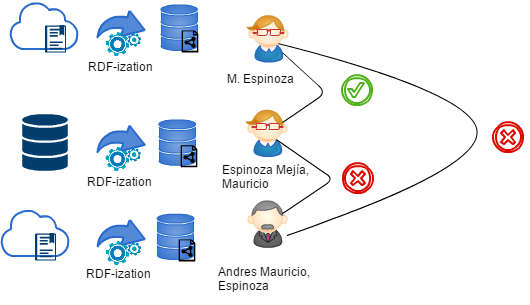
\includegraphics[width=2.5in]{problema}
\caption{Problema de desambiguación}
\label{fig:problema_desambiguacion}
\end{figure}

Los repositorios institucionales a diferencia de las bases digitales de tipo científico  son de naturaleza local, es decir, un repositorio contiene la información generada por una sola institución. Este hecho provoca que generalmente los autores tengan un ámbito reducido de aparición e impacto (institución , ciudad, país ) si se los compara con bases de  ámbito científico que son a nivel global. Otra característica que disponen estos repositorios es que son multidisciplinares, y que abarcan trabajos realizados sobre diferentes áreas de conocimiento tal como matemáticas, economía, ciencias químicas, entre otros. Esta característica  podría aprovecharse en la desambiguación de autores en base a las área de conocimiento en las que trabaja, uesto que es poco probable que un autor con un nombre dado tenga un homónimo que trabaje en el misma área, tal como se concluye \cite{journals/sigmod/FerreiraGL12}.  Debido a las características mencionadas la aplicación de mayoría de métodos de desambiguación existentes podrían verse limitados debido a  requieren de un proceso de análisis particular.

Otra diferencia clara de este tipo de repositorios con respecto a las bases de publicaciones científicas son los metadatos que se emplean para representar los documentos en los repositorios digitales. Por lo general los metadatos que disponen los documentos ingresados en las repositorios digitales son limitados y muy básicos pues su principal objetivo es mantener constancia de cierta documentación, más no un análisis profundo de impacto o de colaboración. La información disponible dentro de los repositorios generalmente dispone de  metadatos generales tales como: título, nombres de los autores, resumen, palabras clave y año de publicación. Por otro lado, información como: afiliaciones y correos de los autores, lugar de publicación o inclusive citas no es considerada. Adicionalmente, hay que considerar que al no existir estándares acordados entre instituciones sobre la calidad de metadatos o definición de términos comunes, es frecuente encontrar errores en esta información. Es por todo esto que la aplicación de algoritmos de desambiguación heredados directamente de las bases digitales no es fiable, desde el punto de vista de la calidad de los metadatos.

Además de las particularidades antes mencionadas la principal característica que diferencia a el caso de uso de los repositorios institucionales respecto a las bases digitales de producción científica  es la distribución de la información de los primeros. Cada institución mantiene su información de manera independiente, a diferencia de las bases digitales que simplemente reúnen el contenido de múltiples fuentes de información en un solo punto de acceso. Es por esto antes de aplicar cualquier enfoque de desambiguación de contenidos, es necesaria la definición de una estrategia de integración de la información de los repositorios. Integración que permita tener una vista unificada de varios repositorios y que a la vez respete la independencia interinstitucional. 

\subsection{Propuesta}
Considerando que el enfoque de desambiguación planteado  considera la independencia y distribución  de las fuentes, se considera la propuesta de arquitectura presentada en \cite{segarra2016integration} como mecanismo de acceso flexible y transparente a la información.  Esta arquitectura requiere que todos los repositorios hayan sido convertidos a datos enlazados (Linked Data) y que puedan ser accedidos a través de los estándares de la web semántica (RDF/SPARQL).

En cuanto al proceso en sí, se establecieron tres etapas principales tal como se presenta en la figura \ref{fig:etapas}, entre las que se destacan las etapas de  Caracterización de los autores, Enriquecimiento semántico y Evaluación. La primera etapa tiene por objetivo, obtener las características más importante de los autores que se van a desambiguar, recopilando desde el repositorio digital afiliación, metadatos de sus documentos y co autores. El enriquecimiento semántico por su parte se encarga de descubrir información relevante a partir de toda la información disponible, detectando tópicos o áreas de interés y filtrando información poco útil. Finalmente en la etapa de evaluación se comparan semánticamente todos los autores (registros ambiguos) en base a varias métricas, lo que permite definir si efectivamente se tratan del mismo individuo. 

\begin{figure}[!t]
\centering
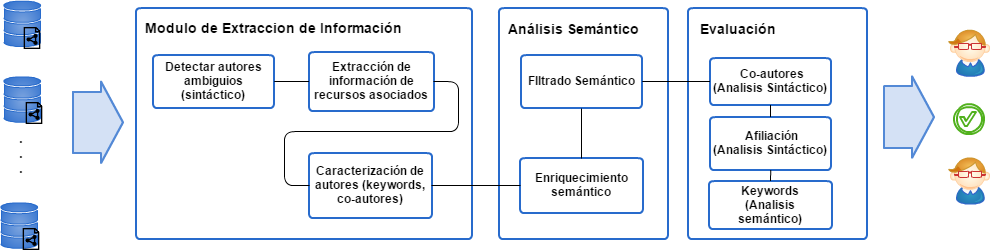
\includegraphics[width=3.5in]{arquitectura}
\caption{Etapas de desambiguaci\'on de autores}
\label{fig:etapas}
\end{figure}

En las siguientes secciones se presentan  a más detalle cada una de las etapas presentadas, especificando los procesos que realizan y las consideraciones que han sido tomadas en cuenta en su desarrollo.  Con el fin de facilitar la comprensión del proceso se ejemplifica cada una de estas etapas con un ejemplo real de ambigüedad de entre autores, encontrado en los repositorios institucionales de las universidades del Ecuador.  Específicamente se tomará al autor ‘Mauricio Espinoza Mejía’, docente e investigador de la Universidad de Cuenca que ha realizado varias colaboraciones con otras instituciones y del cual se conocen varias representaciones ambiguas dentro de los repositorios.

\subsection{Extracción y caracterización de autores}
Para extraer la información de los autores se utilizan los SPARQL Endpoints de cada uno de los repositorios que contienen los datos de los repositorios institucionales en formato RDF. Así mediante consultas simples SPARQL y usando los modelos ontológicos definidos dentro de los repositorios se obtiene una lista de autores para cada repositorio. Adicionalmente, una vez obtenido dicha consulta se completa  la información de los autores obteniendo los metadatos de los  documentos asociados a cada autor y coautores. Toda esta información es asignada a los autores mediante un modelo ontológico simple que se presenta a continuación en la figura \ref{fig:modelo_ontologico}. Adicionalmente, se incluye el nombre del repositorio de origen, información que se utiliza como afiliación del autor.

\begin{figure}[!t]
\centering
%\includegraphics[width=3.5in]{modelo}
\caption{Modelo ontol\'ogico}
\label{fig:modelo_ontologico}
\end{figure}

La lista de autores se obtiene consultando todas las instancias o entidades de la clase persona (foaf:Person) dentro de los repositorios. Esta información se consigue ejecutando el código SPARQL presentado en el segmento de código \ref{lst:seleccion_autores}. Esta consulta proporciona el nombre completo registrado en el repositorio y una URI que sirve de identificador del recurso. En la tabla \ref{tb:autores} se presenta un pequeño extracto de los resultados obtenidos sobre repositorio reales.

\begin{table}[]
\centering
\caption{Autores del repositorio}
\label{tb:autores}
\begin{tabular}{@{}p{0.21\textwidth}p{0.08\textwidth}p{0.1\textwidth}@{}}
\toprule
URI                                                  & Nombre                         & Repositorio           \\ \midrule
UDC:contribuyente/ESPINOZA \_\_MAURICIO               & Espinoza, Mauricio             & Universidad de Cuenca \\
CEDIA:contribuyente/ESPINOZA \_\_MAURICIO             & Espinoza, Mauricio             & CEDIA                 \\
UDC:contribuyente/ESPINOZA \_MEJIA\_\_JORGE\_MAURICIO & Espinoza Mejía, Jorge Mauricio & Universidad de Cuenca \\ \bottomrule
\end{tabular}
\end{table}

\begin{lstlisting}[language=sparql, caption={Consulta para selección de autores.}, label=lst:seleccion_autores, captionpos=b, basicstyle=\footnotesize,frame=single]  
SELECT ?uri ?name {
   ?uri a <http://xmlns.com/foaf/0.1/Person>.
   ?uri <http://xmlns.com/foaf/0.1/name> ?name.
}
\end{lstlisting}

Por otro lado, los metadatos de los documentos asociados a cada uno de los autores y la información de coautores se obtienen mediante la consulta SPARQL presentada en el segmento de código \ref{lst:seleccion_coautores}. Esta consulta debe ejecutarse para cada uno de los elementos de la lista de autores obtenida. En la tabla \ref{tb:coautores} se presenta un ejemplo de los resultados obtenidos para el recurso ‘Espinoza, Mauricio’ del repositorio Universidad de Cuenca.

\begin{lstlisting}[language=sparql, caption={Consulta para selección de coautores.}, label=lst:seleccion_coautores, captionpos=b, basicstyle=\small,frame=single,columns=flexible]  
SELECT ?title ?abtract ?subject ?coauthor {
   ?d <http://purl.org/dc/terms/creator > <%AuthorURI%>.
   ?d <http://purl.org/ontology/bibo/abstract > ?abstract.
   ?d <http://purl.org/dc/terms/title > ?title.
   ?d <http://purl.org/dc/terms/subject > ?subject.
   ?coauthoruri <http://purl.org/dc/terms/creator > ?d.
   ?coauthoruri <http://xmlns.com/foaf/0.1/name> ?coauthor.
   FILTER (str(?coauthoruri) != '%AuthorURI%').
}
\end{lstlisting}

\begin{table}[]
\centering
\caption{Coautores}
\label{tb:coautores}
\begin{tabular}{@{}p{0.1\textwidth}p{0.1\textwidth}p{0.1\textwidth}p{0.1\textwidth}@{}}
\toprule
Título                                                                           & Abstract                                                        & Subjects                                   & Coautores                                             \\ \midrule
RDF-ization of DICOM medical images towards linked health data cloud             & This paper proposes a novel strategy for semantifying DICOM...  & LINKED HEALTH DATA CLOUD, SEMANTICWEB, ... & Andrés Tello, Saquicela Víctor, ...                   \\
Plataforma para la búsqueda por contenido visual y semántico de imágenes médicas & Este trabajo describe una plataforma que permite automatizar... & ONTOLOGÍAS MÉDICAS, SEGMENTACIÓN, ..       & Lizandro Solano, Patricia Gonzalez, Andres Tello, ... \\ \bottomrule
\end{tabular}
\end{table}

Como resultado de esta etapa se obtiene una lista de todos los autores disponibles en todos los repositorios digitales analizados junto con su nombre. Cada autor además posee información de su contexto dentro del repositorio, que consiste en sus coautores, metadatos de sus documentos (título, abstract, Subjects ) y su afiliación (repositorio de origen). Si bien esta información sirve para caracterizar inicialmente a los autores, es necesaria una etapa adicional de procesamiento de información, que será la encargada de disminuir la cantidad de información disponible a procesar,  por una más  pequeña y representativa cantidad de conceptos que caracterizan el trabajo del autor. En la siguiente sección se describe este proceso que es realizado mediante  el análisis, enriquecimiento y filtrado semántico de los documentos.

\subsection{Análisis semántico}

El objetivo de esta etapa consiste en emplear tecnologías semánticas disponibles al momento en función de mejorar la descripción de los datos que representan a un  autor que son obtenidos de la descripciones de los documento.  Para esto se dispone de dos etapas: En la primera se extrae información a partir de los metadatos de los documentos (Título, abstract, subject) mediante el reconocimiento de entidades disponibles en una base de conocimiento como Dbpedia; En segundo lugar se filtra las descripciones basadas en texto obtenidas de pasos anteriores con el objetivo de conservar únicamente aquellas términos que representen mejor el área de trabajo del autor.  Mediante este procedimiento se busca que un autor sea representado  a partir de un número reducido y representativo   de las palabras clave (Subjects y entidades), sus coautores y la institución a la que pertenece tal como se describe a continuación. 

\subsection{Detección de entidades}
Para convertir la descripción de los metadatos de un documento tales como título, palabras clave y abstract , en un número manejable y representativo de información se emplearon técnicas de text mining para la identificación de entidades dentro de los textos (NER- Named Entity Recognition). Las NER  permiten reconocer diferentes tipos de entidades como: localizaciones, personas y conceptos que son referenciadas dentro de un documento o  segmento de texto en las cuales se hacen referencia.  En este caso en particular se utilizó la herramienta Dbpedia Spotlight\footnote{dbpedia-spotlight.org} para la aplicación de esta técnica sobre los documentos, la cual emplea una extensa base de conocimiento como es  Dbpedia\footnote{http://dbpedia.org/} \cite{mendes2011dbpedia}. Mediante la aplicación de esta herramienta se puede descubrir una diversa variedad de entidades dentro de los textos creados de un autor, que además están modeladas como conceptos ontológicos. 

En la tabla \ref{tb:entidades} se presenta un ejemplo de las entidades descubiertas usando Dbpedia Spotlight, para documento ‘Plataforma para la búsqueda por contenido visual y semántico de imágenes médicas’, de autor ‘Mauricio Espinoza’. Nótese que los documentos en español (como es este caso) son traducidos al inglés usando un servicios web de traducción antes de ser analizados con Spotlight. Esto por cuanto el desarrollo de las técnicas NER y de la base de conocimiento (Dbpedia) en sí tienen un mayor desarrollo en su versión en inglés con respecto a otros idiomas y por consiguiente se obtienen mejores resultados.

\begin{table}[]
\centering
\caption{Entidades descubiertas}
\label{tb:entidades}
\begin{tabular}{@{}ll@{}}
\toprule
Segmento de texto & Concepto detectado                                           \\ \midrule
semantic          & http://dbpedia.org/resource/Semantic\_Web                    \\
DICOM             & http://dbpedia.org/resource/DICOM                            \\
medical imaging   & http://dbpedia.org/resource/Medical\_imaging                 \\
ontologies        & http://dbpedia.org/resource/Ontology\_(information\_science) \\ \bottomrule
\end{tabular}
\end{table}

\subsection{Filtrado semántico}
En la mayoría de documentos las palabras clave tomadas de los metadatos y las entidades extraídas a partir los abstract representan las áreas de interés de un autor, sin embargo, existen otros casos donde más bien pueden llegar producir errores e inconsistencias. Por ejemplo, muchas de las palabras clave ingresadas en los metadatos de documentos incluyen referencias a localizaciones  e instituciones como: Provincia del Azuay o Hospital Regional Vicente Corral, etc. También es común que se incluyan categorizaciones propias de la universidad como: Tesis de pregrado, Tesis de maestría, etc. Estas referencias no ayudan a distinguir entre autores, sino que al contrario pueden introducir ruido al proceso de comparación. Por otro lado, las entidades reconocidas mediante NER también son susceptibles a errores, en especial cuando los texto son cortos. Un ejemplo de ambigüedad introducida por el proceso NER es la definición de las siglas, así en ciertos casos ‘NGD’ que puede tomar el significado de ‘Normalized Google Distance’ (Contexto informático) cuando en realidad puede referirse a ‘Non-Good Delivery’ (Contexto  de manipulación de barras de oro). Es por todo esto que se implementó una actividad de filtrado semántico de las palabras clave, que está pensada en mejorar la calidad de las palabras clave que representan un autor.

La primera parte del proceso de filtrado utiliza una lista de palabras vacías (stopwords), la cual se descubrió tras un análisis de las palabras clave usadas en los metadatos de los documentos. Esta lista identifica términos comunes para referirse a localizaciones e instituciones como: “Cantón”, “Provincia”, “Hospital”, etc. Cuando uno de estos términos es encontrado, se desecha toda la palabra clave del proceso de desambiguación. Por ejemplo la palabra clave “Cantón Cuenca - Azuay” es ignorada puesto que contiene la palabra vacía “Cantón”. Adicionalmente, los entidades descubiertas con Dbpedia Spotlight que se identifiquen como una localización geográfica (clase Dbpedia:Place) también son ignoradas, lo que se consigue consultado el SPARQL Endpoint de Dbpedia. Esta primera fase de filtrado permite eliminar referencias inútiles del proceso de desambiguación y que por el contrario pueden introducir ruido al proceso.

La segunda y última parte del proceso de filtrado semántico consiste en eliminar las palabras clave que tengan menor relevancia semántica respecto las keyword obtenidas de los trabajos de un autor. Esto se consigue evaluando la similitud semántica entre cada una de las palabras clave con respecto a las demás del conjunto, permitiendo  determinar qué tan relacionadas están las palabras clave entre sí. Aquellas palabras que presenten menor relación semántica con respecto a las demás serán consideradas como ruido, con lo cual es posible  eliminar posibles conceptos detectados de forma errónea o palabras clave que no aporten a la identificación del área de trabajo de un autor.

Para la implementación de este filtrado se empleó la medida de relación semántica NWD (Normalized Wikipedia Distance) \cite{schaefer2014normalized}, debido a que presentó mejores resultados al relacionar semánticamente palabras con respecto a técnicas que empleaban como base de conocimiento WordNet \cite{kilgarriff2000wordnet} o similares. WND es una métrica simple que evalúa la distancia semántica entre dos cadenas de texto, mediante la operaciones de búsqueda (Full-text). NWD es una adaptación de NGD (Normalized Google Distance) \cite{DBLP:journals/corr/abs-cs-0412098} que opera sobre Wikipedia como base de conocimiento en lugar del motor de búsqueda de Google. Esta métrica ofrece una gran flexibilidad puesto que no requiere de vocabularios fijos ni información previamente estructurada para su utilización, como sí lo hacen la mayoría de métricas disponibles en el estado del arte. En el segmento de código \ref{eq:nwd} se presenta la fórmula utilizada para evaluar NWD, la misma que es implementada sobre la API de búsqueda de Wikipedia\footnote{https://www.mediawiki.org/wiki/API:Search}.

\begin{equation} \label{eq:nwd}
NWD(x,y)  = \frac{\max(\log{f(x)},log{f(y)})-\log{f(x,y)}}{\log{N}-\min(\log{f(x)},\log{f(y)})} \\
\end{equation}
$f(t)$: Número de resultados al buscar t en Wikipedia.\\
$N$: Número total de artículos de Wikipedia.\\
$f(t,u)$: Número de resultados al buscar t y u en Wikipedia.


La evaluación de la similitud entre los palabras clave se realiza mediante la sumatoria de la distancia de una palabra clave con respecto a las demás palabras del conjunto. Propiamente si un autor posee las palabras clave $p1, p2, … pn$, la relevancia(rn) de cada una de las palabras clave se estima mediante la fórmula presentada en en el segmento de código \ref{eq:relevancia}. Nótese que al tratarse de distancias semánticas las palabras clave que obtengan menor valor ($r$) se consideran más relevantes para un autor.

\begin{equation}\label{eq:relevancia}
r(i) = \sum_{j!=i}^{j<n} NWD(p_i, p_j)
\end{equation}

El criterio seguido para definir el número de palabras clave que deban sobrepasar el filtro se definió mediante una regla práctica basada en las observaciones realizadas sobre los datos. Se definió que para un conjunto N de palabras clave se debería seleccionar (2*ln N) palabras más relevantes para ser usadas por la siguiente etapa. Esta regla ofrece un crecimiento amortiguado del número de palabras clave a ser usados, de manera que autores con pocas palabras clave no las pierdan debido al filtrado semántico y al mismo tiempo que autores con demasiadas palabras clave limiten el número de estas.

\section{Evaluación y Resultados}
\label{sec:evaluacion_resultados}

\begin{figure}[!t]
\centering
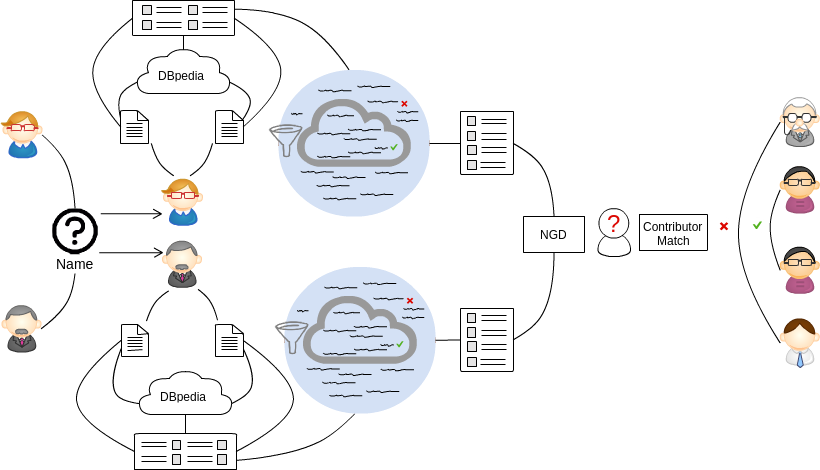
\includegraphics[width=0.5\textwidth]{proceso}
\caption{Comparaci\'on entre autores}
\label{fig:comparacion}
\end{figure}

Como se presenta en la figura \ref{fig:comparacion} la comparación final entre los autores y descubrimiento de enlaces entre estos se realiza en dos etapas. En la primera etapa se determinan autores candidatos que podrían tratarse del mismo individuo a través de la detección de nombres similares. En la segunda se realiza una comparación semántica entre los candidatos con la información obtenida luego del proceso de análisis semántico (Afiliación, coautores y palabras clave). Finalmente, los candidatos que superen un umbral mínimo de distancia semántica son considerados equivalentes y se crean enlaces para estos. A continuación se detallan estas dos etapas con las métricas que utilizan.

\subsection{Autores candidatos}
Existe un gran variedad de algoritmos para evaluar la similitud sintáctica entre dos cadenas de texto, sin embargo, los algoritmos basados en Tokens son los más utilizados para la detección de nombres similares. Estos algoritmos representan los nombres como conjuntos de palabras (tokens) y aplican operaciones de conjuntos para determinar su similitud. Ejemplos típicos de estos algoritmos usados en la comparación de nombres son Jaccard, Overlap, tal como se trata en  \cite{huynh2013vietnamese}. No obstante, para cubrir de manera más general este problema es necesario agregar más características a estas métricas con el fin de hacerlas más flexibles a particularidades comunes en los nombres de personas como: Iniciales y abreviaturas \cite{shoaib2015improving}.

En presente se plantea la utilización de una métrica híbrida que utiliza los enfoques de tokens, similitud de texto simple y manejo e iniciales y abreviaturas. Específicamente se plantea usar una versión adaptada de Jaccard para la comparación de nombres. Que se complementa con la  métrica de ‘Jaro-Winkler’ para la generación de  match flexibles entre tokens que trate problemas de iniciales y abreviaciones de los nombres. En el segmento de código \ref{eq:metrica} se presenta esta métrica de forma más formal.

\begin{equation}\label{eq:metrica}
NamDis(N1, N2) = \frac{MJW(N1, N2)+ MAI(N1,N2)}{N}
\end{equation}
$MJW$: Número matchs entre las palabras (tokens) de los nombres $N1$ y $N2$ usando la métrica Jaro-Winkler con un umbral de $0.95$.\\
$MAI$: Número de matchs entre las palabras (tokens) de los nombres $N1$ y $N2$, tomando iniciales y abreviaturas. (Ignorando las palabras usadas en los matchs de $MJW$)\\
$N$: Número total de tokens en $N1$ y $N2$.

Para la detección la lista de autores candidatos a ser desambiguación se aplica esta métrica entre todos los autores detectados en los repositorios. Los pares de autores que sobrepasen un umbral de similitud del nombre de $0.8$  se agregan a la lista de candidato a desambiguar.

\subsection{Comparación semántica}
La comparación de candidatos se realiza en tres partes:  afiliación, coautores y palabras clave. Para cada una se han definido métricas simples  que aportan conocimiento de la relación entre los candidatos. Al finalizar la evaluación de cada una estas se genera un índice único calculado a partir de las tres métricas, el cual se utiliza para determinar si se trata o no del mismo autor.   A continuación se explica cada una de las partes de esta comparación.

El factor de afiliación (FA) es el más simple de todos, simplemente si dos autores candidatos tiene la misma afiliación (pertenecen a la misma institución) el factor toma el valor de 0.9, caso contraro de 1 es asignado. Esta condición se basa en la suposición que si encontramos autores candidatos en un mismo repositorio es más probable que se traten de la misma persona. Si bien esta suposición puede parecer sesgada cuando se ve desde el punto de vista de bases digitales u otras fuentes de información, en realidad se elaboró considerando la naturaleza local de los repositorios digitales.
 
El factor de coautores (FC) por su parte se activa cuando el nombre de al menos un coautor de los dos candidatos es el mismo, en este caso FC pasa a ser 0.9, caso contrario se mantiene en 1. Esta regla se basa en el principio que si dos candidatos comparten coautores es muy probable que se trate del mismo individuo. Hay que destacar que para evaluar la similitud de los nombre de los coautores se utiliza la misma métrica definida para descubrir los autores candidatos. Este tipo de suposiciones es muy común en los algoritmos de desambiguación usados en bases digitales porque mejora notablemente la precisión de los algoritmos.

El índice de similitud de palabras clave (ISPC) entre los candidatos se define como el promedio de las distancias entre todas las palabras clave usando NWD. Este índice está pensado para reflejar cual es la distancia semántica entre los temas de interés de los candidatos. Donde una distancia menor signifique que tratan temáticas parecidas y una distancia mayor implique temas de investigación distintos. En el segmento de código \ref{eq:distancia} se presenta formalmente la definición de la distancia entre dos cándidos (A1, A2) con los conjuntos de  palabras clave $P1$ y $P2$.

\begin{equation}\label{eq:distancia}
ISPC(A1,A2) = \frac{\sum_i^{i<P1N}\sum_j^{j<P2N}NWD(P1_i, P2_j)}{P1N*P2N}
\end{equation}
$P1N$: Es el número de palabras clave en $P1$.\\
$P2N$: Numero de palabras clave en $P2$.

Finalmente, la distancia total ponderada (DTP) se define como $DTP= FA*FC*ISPC$. Distancia que resume toda la información de dos autores y su cercanía semántica entre sí. A partir de este índice se aplica un filtrado simple con un umbral de 0.7. De manera que todos los pares de autores candidatos con un índice DTP menor a 0.7 son considerados el mismo individuo y por tanto enlazados a través de enlaces (sameAs).


\section{Conclusión y trabajos futuros}
\label{sec:conclusion}
La desambiguación de autores es una problemática común en todos los sistemas de información bibliográfica y que por su importancia ha recibido especial atención de la comunidad de investigadores. Sin embargo, la mayor parte de lo esfuerzos investigativos se han centrado en solucionar los problemas de ambigüedad en bases de digitales de producción científica dejando   en segundo plano a otros sistemas como los repositorios digitales. En este contexto surge la necesidad de atraer la investigación a este tipo de fuentes de información, adaptando las técnicas existentes de desambiguación a este nuevo entorno.

En este trabajo se presenta un nuevo proceso de desambiguación semántica de autores aplicado al contexto de los repositorios digitales. Proceso que considera las particularidades de este tipo de sistemas de información y adapta técnicas semánticas de vanguardia como: reconocimiento de entidades, métricas de similitud semántica y bases de conocimiento ontológicas. Adicionalmente, el enfoque de desambiguación presentado se enmarca en las principios de Datos enlazados y Web Semántica lo que amplía su ámbito de aplicación a la Web. 
Adicionalmente, los resultados obtenidos están limitados a ciertas suposiciones, que podrían afectar al rendimiento del algoritmo, tales como:  Los obras están correctamente asignadas a sus autores, por lo que no se considera el problema de reasignación de obras; No existen autores con nombres similares que  dispongan de obras sobre  áreas similares;  Los autores carecen de identificadores únicos por lo que no son considerados en este contexto.

El trabajo futuro se centrará en el mejoramiento del proceso de desambiguación planteado mediante la explotación de estructuras ontológicas que utilizan la bases de conocimiento (jerarquías, clasificaciones de conceptos, etc). Estas mejoras estarán orientadas a cubrir nuevas y más complejas fuentes de información, así como refinar los resultados obtenidos. Finalmente, se propone expandir la utilidad de los algoritmos desarrollados en este trabajo para atacar otras problemas comunes en los sistemas bibliográficos y de manejo de autores como  catalogación automática de documentos e identificación de redes de colaboración entre autores.

\section*{Acknowledgment}
Al Consorcio Ecuatoriano para el Desarrollo de Internet Avanzado (RED-CEDIA), por el financiamiento brindado a esta investigación, mediante el proyecto “Repositorio Semántico de Investigadores del Ecuador” y el grupo de trabajo de Repositorios Digitales. Adicionalmente, al Departamento de Ciencias de la Computación de la Universidad de Cuenca.


% trigger a \newpage just before the given reference
% number - used to balance the columns on the last page
% adjust value as needed - may need to be readjusted if
% the document is modified later
%\IEEEtriggeratref{8}
% The "triggered" command can be changed if desired:
%\IEEEtriggercmd{\enlargethispage{-5in}}

\bibliographystyle{IEEEtran}
\bibliography{IEEEabrv,bibliografia}
\end{document}


